%!TEX root = ../Thesis.tex
%IntroductionPartI

\chapter*{Introduction to Part I}
\addcontentsline{toc}{chapter}{Introduction to Part I}
\label{IntroductionPartI}
\lhead{Introduction to Part I} % Write in your own chapter title to set the page header

The current interest to develop new quantum technologies is boosting applied
and fundamental research on quantum phenomena and systems with potential
applications in logic circuits, metrology, communications or sensors. Robust basic
devices performing elementary operations are needed to perform complex tasks
when combined in a circuit. With the goal of increasing the knwoledge in quantum technologies and making proposals for new applications of quantum physics, in this chapter I will approach the design of devices that control the flow of quantum particles in an asymmetric way. In order to achieve this I will investigate the properties of potentials with asymmetric
transmission or reflection for a quantum, spinless particle of mass $m$ satisfying a one-dimensional (1D) Schr\"odinger equation.

We propose six different types of asymmetric devices, see fig. \ref{cases}. The six types of devices are classified according to the transmission and reflection coefficients of the scattering potentials, which in the ideal case would take only values of 0 or 1. For example, the device in fig. \ref{cases}(a), called \textit{One-way mirror} ($\cal{TR/A}$) reflects back and transmits incoming wave packets with the same intensity for left incidence, whereas all the wave packets coming from the right are completely absorbed. In fig. \ref{cases}(c) the \textit{One-Way T-filter} ($\cal{T/A}$) would be the equivalent to a diode, since it transmits all the wave packet for left incidence while it behaves as an insulator for right incidence.

\begin{figure}
  \center
  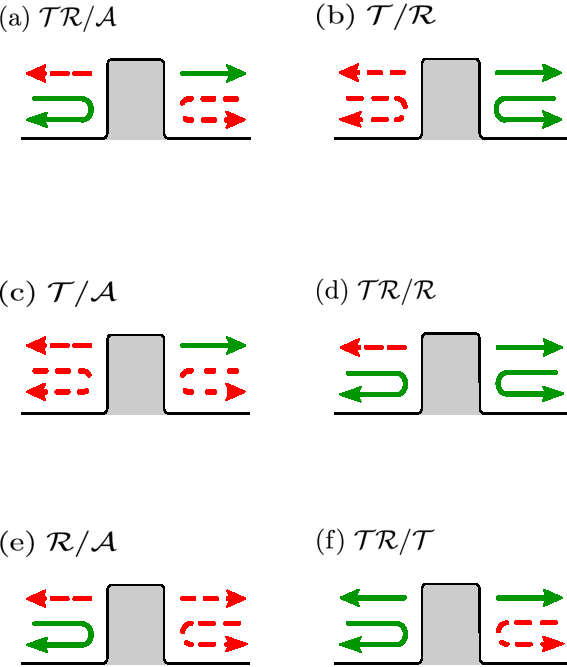
\includegraphics[width = 0.5\linewidth]{Figures/PotentialCasesPT.pdf}
  \caption{Devices with asymmetric scattering (limited to scattering coefficients being 0 or 1).  The dashed and continuous lines represent respectively zero or one
  for the moduli of the scattering amplitudes; the bended lines are for reflection amplitudes, and the straight lines for transmission:
  (a) One-way mirror ($\cal{TR/A}$); (b) One-way barrier ($\cal{T/R}$); (c) One-Way T-filter ($\cal{T/A}$);
  (d) Mirror \& 1-way transmitter ($\cal{TR/R}$); (e) One-way R-filter ($\cal{R/A}$); (f) Transparent, one-way
  reflector ($\cal{TR/T}$).
  The letter codes summarize the effect of left and right incidence, separated by a  slash ``$/$''.
  ${\cal T}$ or ${\cal R}$ on one side of the slash indicate a unit
  transmission or reflection coefficient
  for  incidence from that side, whereas the absence of one or the other letter corresponds to zero coefficients.
  An ${\cal A}$ denotes ``full absorption'', i.e., both moduli of reflection and transmission amplitudes are zero for incidence from one side.
  For example,  $\cal{TR/A}$ means unit modulus transmission
  and reflection from the left and total absorption from the right.
  \label{cases}}
\end{figure}

As we shall see in the following chapters, the asymmetric devices in fig. \ref{cases} cannot be constructed with Hermitian Hamiltonians/potentials \cite{Muga2004,Mostafazadeh2018}. Some of them even require the potential not being local. Thus  non-local, and non-Hermitian potentials are needed to implement a rich set of scattering asymmetries, and in particular asymmetric transmission.

Although nonlocal and nonhermitian potentials may seem uncommom and extraordinary in quantum physics, they appear naturally when applying partitioning techniques to describe the effective interactions in a subspace of a larger system with a Hermitian Hamiltonian by projection \cite{Feshbach1958,Ruschhaupt2004,Muga2004}. Non-Hermitian (NH) Hamiltonians representing effective interactions have a long history in nuclear, atomic, and molecular physics, and have become common in optics, where wave equations in waveguides could simulate  Schr\"odinger equations \cite{Ruschhaupt2005,Longhi2017a,Konotop2016}. NH Hamiltonians can also be set phenomenologically, e.g. to describe dissipation \cite{Ruschhaupt2005}.

Recently there has also been a lot of interest in Non-Hermitian Hamiltonians \cite{Nixon2016,Nixon2016a,Chen2017,Ruschhaupt2017,Simon2018,Simon2019a,Alana2020,Bernard2002,Kawabata2019}. In particular, the ones having parity-time (PT) symmetry \cite{Bender1998,Znojil2015} because of their spectral properties and useful applications, mostly in optics  \cite{Longhi2017a,Konotop2016,Longhi2014}. As happens with Hermitian Hamiltonians, symmetry operations on NH Hamiltonians can be systematized into group structures \cite{Ruschhaupt2017,Simon2019a,Alana2020}. In particular for
1D scattering potentials, the different Hamiltonian symmetries imply
selection rules for asymmetric transmission and reflection \cite{Ruschhaupt2017,Simon2019a} that will pose limitations to the design of the asymmetric devices in fig. \ref{cases}.
%

The contents of this part of the thesis will be organized as follows. In chapter \ref{Chapter1} I will give a brief introduction to the theory of scattering in one dimension by non-hermitian potentials. Next, I will describe the set of asymmetric devices and the different selection rules imposed by the set of symmetries formed by parity, time-reversal and PT. In chapter \ref{Chapter2} I will further investigate an extended symmetry group on the Hamiltonians that will have interesting consequences on the eigenvalues. In chapter \ref{Chapter3} I discuss possible physical implementations of non-local and non-hermitian potentials with 3-level atoms interacting with laser fields.
